\Subhead{5.1.4}{Фазированные антенные решётки}

В линейной решётке $N$ одинаковых элементов с шагом $d$ и возбуждениями $a_n\e^{\ii n\psi}$ зададим положения $\bm r_n=nd\bm e_x$ и ориентированный угол $\widehat{\bm r}\cdot\bm e_x=\sin\theta$. При временной зависимости $\e^{-\ii\omega t}$ и исходящей волне $\e^{\ii kr}$ имеем $|\bm r-\bm r_n|\simeq r-nd\sin\theta$. Дальнее поле равно произведению диаграммы элемента на множитель решётки:
\begin{equation}
 AF(\theta)=\sum_{n=0}^{N-1}a_n\e^{\ii n(\psi-kd\sin\theta)}.
\end{equation}
Угол отсчитывается от нормали с указанным положительным направлением. При равных амплитудах сумма геометрической прогрессии даёт $|AF|=|\sin(Nu/2)/\sin(u/2)|$, $u=\psi-kd\sin\theta$. Главный максимум направляется условием $\psi-kd\sin\theta_0=0$ по модулю $2\pi$. Фазовое управление поворачивает луч без механического движения.

Ширина главного лепестка по порядку $\lambda/(Nd\cos\theta_0)$; амплитудное взвешивание уменьшает боковые лепестки ценой расширения. Другие решения $u=2\pi m$ могут дать решёточные лепестки. Строгое отсутствие дополнительного решёточного максимума на всём замкнутом диапазоне требует $d<\lambda/2$. При $d=\lambda/2$ крайнее наведение на $+90^\circ$ даёт такой же фазовый максимум и на $-90^\circ$; обычная запись $d\leq\lambda/2$ исключает эти крайние положения. При ограниченном сканировании возможны более крупные шаги. Фиксированные фазовращатели создают частотно-зависимое направление луча, а истинные временные задержки уменьшают этот эффект. Взаимное влияние элементов и их согласование нарушают простую модель произведения.
\begin{center}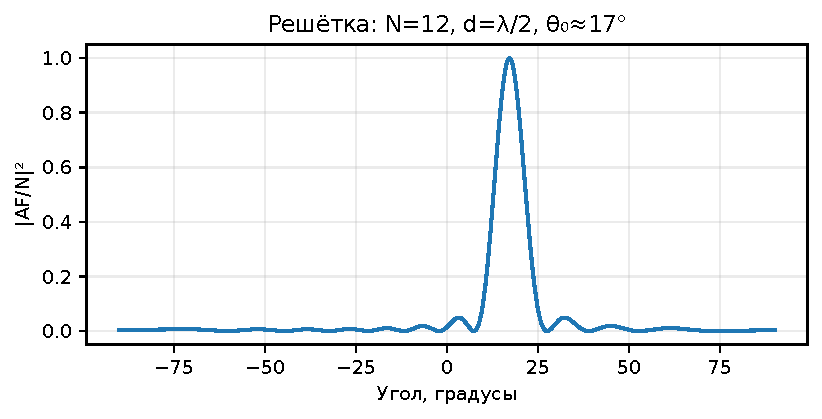
\includegraphics[width=0.82\linewidth]{figures/array.pdf}\end{center}

